
\documentclass[../main.tex]{subfiles}

\begin{document}

Our results demonstrate that LeafAI is capable of rivaling the ability of a human programmer in matching patients eligible to clinical trials. Indeed, in numerous cases we found LeafAI and the human programmer executing similar queries, such as for Hepatitis C (NCT04852822), Chronic Lymphocytic Leukemia (NCT04852822), Multiple Sclerosis (NCT03621761), and Diabetes Mellitus (NCT03029611), where both ultimately matched a similar number of patients.

One notable pattern we found is that LeafAI consistently finds a higher number of potentially eligible patients. We hypothesize that in many cases, LeafAI's KB played a key role both in finding additional eligible patients, but also sometimes in unnecessarily excluding otherwise eligible patients. For example, in the Multiple Sclerosis (MS) trial, LeafAI searched for 11 different SNOMED codes related to MS (including MS of the spinal cord, MS of the brain stem, acute relapsing MS, etc.), while the human programmer searched for only one, and ultimately LeafAI found nearly 5 times the number of potentially eligible patients (4,891 versus 1,016). We further hypothesize that the human programmer likely had a lower rate of false positives (and thus higher precision), though we leave an analysis of that to future work. On the other hand, in the same trial, as can be seen in Figure \ref{fig_leafai_results_analysis}, given the exclusion criteria: "Current shift work sleep disorder, or narcolepsy diagnosed with polysomnography and multiple sleep latency", LeafAI's KB included diagnosis codes for drowsiness, snoring, and so on, as within the UMLS they appear as child concepts of sleep disorder (C0851578). The exclusion of these patients likely resulted in an approximately 40\% drop in recall at that stage compared to the human programmer, though ultimately both achieved similar recall (39\% versus 35\%). Though outside the scope of the current project, in future work we intend to review subsets of patients found by LeafAI to determine their eligibility statuses. 

Beyond performance as measured by recall, it is notable that the human programmer spent approximately 26 hours crafting queries for the 8 trials while LeafAI took only several minutes running on a single laptop. The time saved by using automated means such as LeafAI for cohort discovery may save health organizations significant time and resources.

\subsection*{Limitations}

This project has a number of limitations. First, while the 8 clinical trials we evaluated were randomly selected, we specifically restricted the categories of diseases from which trials were chosen and limited to trials with 30 or less lines of eligibility criteria, and thus our results may not generalize to other kinds of trials. Next, we evaluated our queries using an OMOP-based extract which did not contain the full breadth of data within our EHR. Had our experiments instead been conducted using our enterprise data warehouse (populated by our EHR), it is possible the human programmer would have achieved greater results than LeafAI due to knowledge and experience in utilizing granular source data. For example, in the Cardiac Arrest clinical trial, the human programmer noted that data for use of cooling blankets is available in our EHR, but not in OMOP. It is not clear how LeafAI would perform were such data available. We further did not directly compare to other NLP systems. While we considered evaluating another notable system, Criteria2Query \cite{yuan2019criteria2query}, as part of our baseline, we ultimately determined it inappropriate for our analysis as we aimed to review results longitudinally (i.e., line by line of criteria), a function which Criteria2Query was not designed for. 

\subsection*{Future work}

We are actively developing a web-based user interface for LeafAI, shown in Figure \ref{fig_leafai_screenshot}. In future work, we will deploy a prototype of the tool and evaluate user feedback and system performance. The LeafAI web application will provide rapid feedback to users explaining its search strategies, and allow users to override system-reasoned concepts and edit or add their own. Additionally, we intend to explore the adaptation of our logical form-based query generation methods to general-purpose question answering and querying systems such as FHIR endpoints.

\begin{figure}[H]
  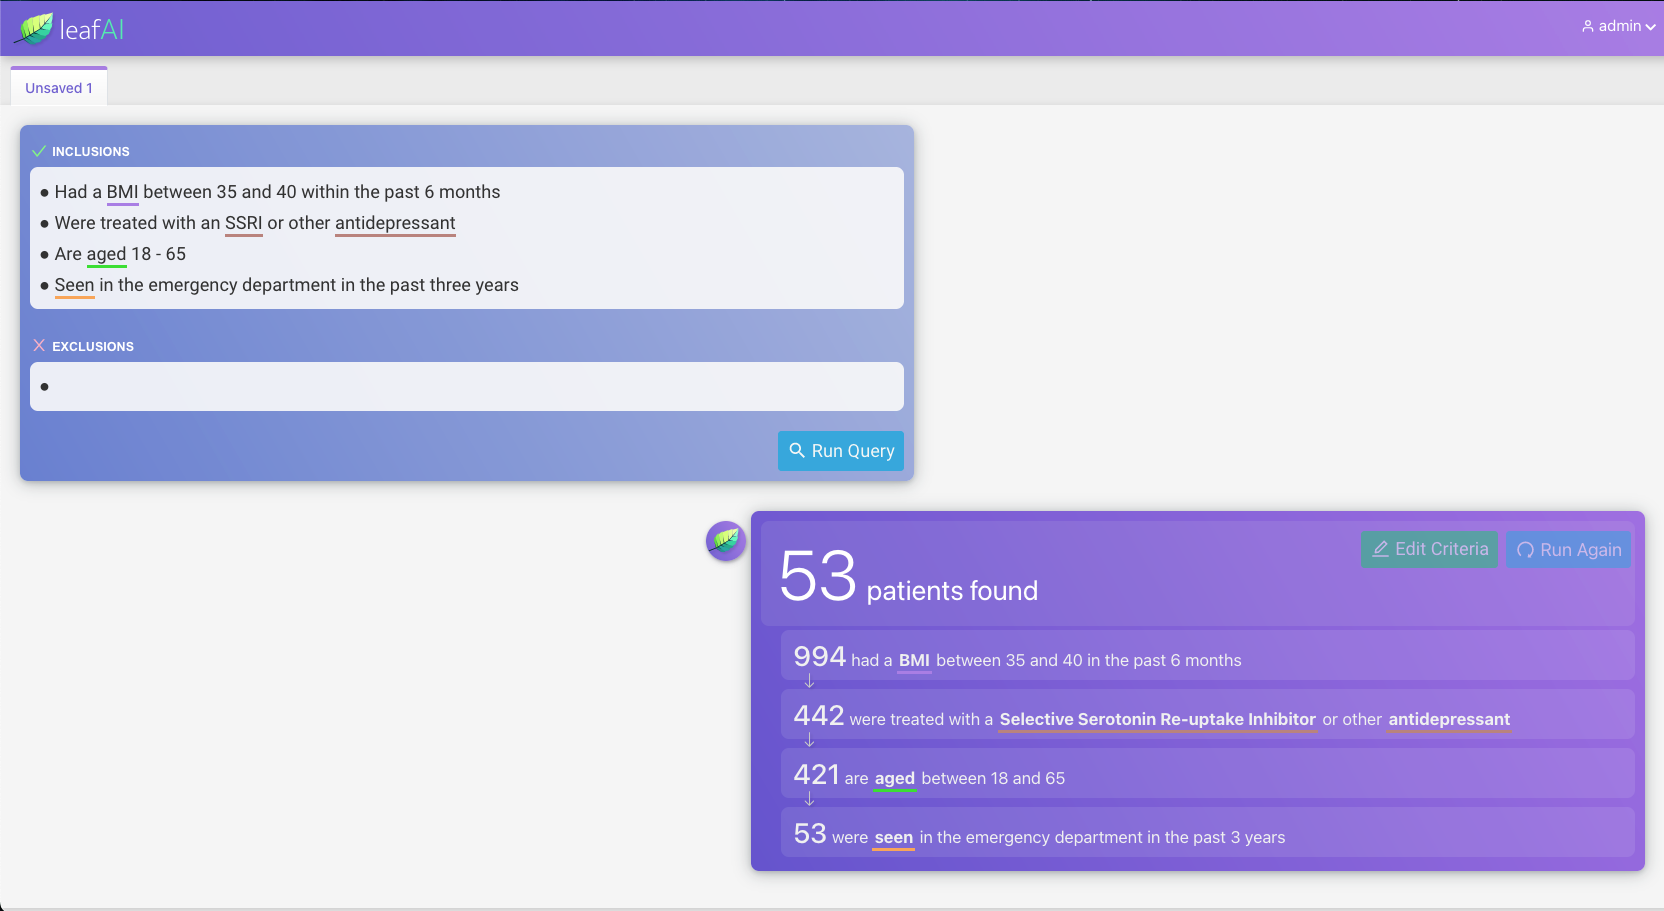
\includegraphics[scale=0.26]{figures/leafai_screenshot.png}  
\caption{Example screenshot of the LeafAI web application, which is currently in development.}
\label{fig_leafai_screenshot}
\end{figure}

\end{document}